\documentclass[10pt]{article}
\usepackage[utf8]{inputenc}
\usepackage[doublespacing]{setspace}
\usepackage{textcomp}
\usepackage{amsmath,amssymb,amsthm}
\usepackage{fancyhdr}
\usepackage{lastpage}
\usepackage[]{hyperref}
\usepackage[pdftex]{graphicx}
\usepackage{ctex}
\usepackage{booktabs}
\usepackage{subfigure}
\usepackage{titlesec}
\usepackage{listings}
\usepackage{enumerate}
\usepackage{bm}
\usepackage{float}
\usepackage{url}
\usepackage[english]{babel}
\usepackage[dvipsnames]{xcolor}
\usepackage{scalerel}
\usepackage[margin=1.25in]{geometry}
%\allowdisplaybreaks
\renewcommand{\contentsname}{\centerline{Contents}}
\pagestyle{fancy}
\author{D}
\def\name{D}
\lhead{Multivariate Statistical Methods}
\chead{}
\rhead{\name}
\cfoot{-\space\thepage\space-}
\newtheorem{prob}{\bm{$Problem$}}
\newtheorem{bonus}{\bm{$Bonus\;Problem$}}
\newcommand{\tabincell}[2]{\begin{tabular}{@{}#1@{}}#2\end{tabular}}
\CTEXoptions[today=old]

\begin{document}

\title{Assignment Three}
\date{\today}
\maketitle
\thispagestyle{fancy}
\vspace{3mm}

\newpage

\begin{prob}
\end{prob}
\begin{enumerate}[1)]
\vspace{3mm}

\item
Using R, we perform the principal component analysis (PCA) on the correlation matrix $\pmb{\rho}=
  \begin{bmatrix}
    1 & -0.01\\
    -0.01 & 1
  \end{bmatrix}$
. We get the following outputs.\footnote{\;csgillespie. (2010, July 19). Answer to PCA on correlation or covariance. In \textit{Stack exchange}. Retrieved 7:13, May 21, 2020, from \url{https://stats.stackexchange.com/questions/53/pca-on-correlation-or-covariance}.}\\
\begin{table}[H]
\centering
\begin{tabular}{|c|cc|}
\hline
Variable   & PC1   & PC2  \\ \hline
{\fontfamily{ptm}\ttfamily SkiJump}      & -0.71 & 0.71 \\
{\fontfamily{ptm}\ttfamily CrossCountry} & 0.71  & 0.71 \\ \hline
\end{tabular}
\caption{Loadings for the two PCs}
\end{table}
With {\fontfamily{ptm}\ttfamily summary} in R, we get that PC1 explains 50.53\% of the total variation and PC2 explains 49.47\% of it. The two PCs explain 100\% of the total variation.\\
Let $x$ and $y$ denote the values of {\fontfamily{ptm}\ttfamily SkiJump} and {\fontfamily{ptm}\ttfamily CrossCountry} respectively and a number represent the item number. Use {\fontfamily{ptm}\ttfamily biplot}.
\begin{figure}[H]
  \centering
  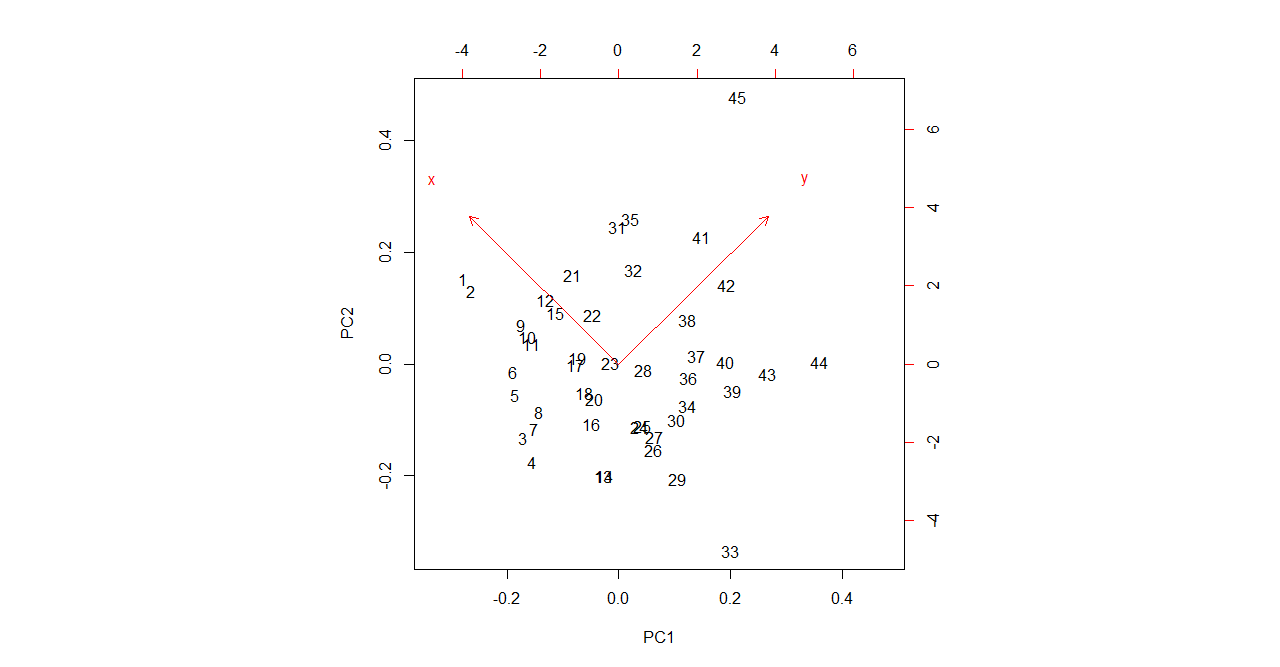
\includegraphics[scale=0.4]{p1b.png}
  \caption{PCA plot}
\end{figure}

\item
The reason is that this way reduces the dimensionality of the transformed data, by using one score instead of two numbers, making the score easily computed and interpreted and able to difference the athletes.

\item
First of all, since the two variables are on different scales, we need to turn the data into PCA data on the same scale. We do this with matrix calculation.\\
We define a new column {\fontfamily{ptm}\ttfamily PC1 scores}, computed by $(x,PC1)\times x+(y,PC1)\times y$, and sort this column in a descending order. We find the person, Lukas Runggaldier from Italy, is the third one and wins the bronze medal.\footnote{\;Carr. S. M. (2001). \textit{Interpreting a principal components analysis - theory \& practice}. Retrieved 9:30, May 21, 2020, from \url{http://www.mun.ca/biology/scarr/2900_PCA_Analysis.htm}.}

\item
The second principal component explains 49.47\% of the total variation. It is computed by $0.71\times x+0.71\times y$. Since {\fontfamily{ptm}\ttfamily CrossCountry} measures time, the smaller it is the better the score should be. Hence, a good PC2 score represents a good {\fontfamily{ptm}\ttfamily SkiJump} value and a bad {\fontfamily{ptm}\ttfamily CrossCountry} value. Using this score will encourage athletes to perform well at ski jumping and discourage them at cross-country skiing.

\item
No, since each component explains only around half of the total variation, if we use 80\% as a threshold for cumulative proportion to summarize the data, neither of them can solely summarize the data adequately.

\item
No, with the correlation matrix $\pmb{\rho}=
  \begin{bmatrix}
    1 & -0.01\\
    -0.01 & 1
  \end{bmatrix}$
, we observe there is very weak negative correlation between {\fontfamily{ptm}\ttfamily SkiJump} and {\fontfamily{ptm}\ttfamily CrossCountry}. {\fontfamily{ptm}\ttfamily SkiJump} and {\fontfamily{ptm}\ttfamily CrossCountry} are almost independent and thus not equivalent.

\item
No, since we tend to perform the PCA on the covariance matrix when the variable scales are similar and on the correlation matrix when variables are on different scales,\footnote{\;csgillespie. (2010, July 19). Answer to PCA on correlation or covariance. In \textit{Stack exchange}. Retrieved 7:13, May 21, 2020, from \url{https://stats.stackexchange.com/questions/53/pca-on-correlation-or-covariance}.} {\fontfamily{ptm}\ttfamily SkiJump} is the ski jump score and {\fontfamily{ptm}\ttfamily CrossCountry} is the cross-country time in seconds, so they are on different scales and we do not suggest perform the PCA on the covariance matrix.\\
If we use only the first principal component on the covariance matrix to compute the score, with the same step in A.3, we get that Alessandro Pittin from Italy is the first one and wins the gold medal. In PC1, the coefficient for {\fontfamily{ptm}\ttfamily SkiJump} is -0.0014 and the coefficient for {\fontfamily{ptm}\ttfamily CrossCountry} is 0.9999, so the score is almost determined only by {\fontfamily{ptm}\ttfamily CrossCountry}.

\end{enumerate}
\vspace{6mm}

\begin{prob}
\end{prob}
\begin{enumerate}[1)]
\vspace{3mm}

\item
Five. Use {\fontfamily{ptm}\ttfamily factanal} in R, we get that when number of factors is 5, the p-value is 0.071 and starts to be greater than the threshold 0.05.

\item
With R, we get the factor loadings table.
\begin{table}[H]
\centering
\small
\begin{tabular}{|c|ccccc|}
\hline
Variable & Factor1 & Factor2 & Factor3 & Factor4 & Factor5 \\ \hline
{\fontfamily{ptm}\ttfamily REACT}    & 0.782  &        &        &        &        \\
{\fontfamily{ptm}\ttfamily HEIGHT}   & 0.176  & 0.888  & -0.164 & 0.189  &        \\
{\fontfamily{ptm}\ttfamily WEIGHT}   & 0.614  & 0.615  & -0.187 & 0.424  &        \\
{\fontfamily{ptm}\ttfamily SHLDR}    & 0.193  & 0.747  & -0.146 & 0.100  & -0.247 \\
{\fontfamily{ptm}\ttfamily PELVIC}   & 0.238  & 0.585  & -0.272 & 0.195  &        \\
{\fontfamily{ptm}\ttfamily CHEST}    & 0.488  & 0.458  & -0.112 & 0.666  & -0.121 \\
{\fontfamily{ptm}\ttfamily THIGH}    & 0.957  & 0.104  & -0.117 &        &        \\
{\fontfamily{ptm}\ttfamily PULSE}    & -0.114 & 0.575  & 0.146  &        &        \\
{\fontfamily{ptm}\ttfamily DIAST}    & -0.166 & 0.230  & 0.166  & 0.142  &        \\
{\fontfamily{ptm}\ttfamily CHNUP}    & -0.690 & -0.175 & -0.109 & -0.124 &        \\
{\fontfamily{ptm}\ttfamily BREATH}   & 0.166  & 0.598  & 0.145  &        &        \\
{\fontfamily{ptm}\ttfamily RECVR}    & 0.102  & 0.948  & -0.127 & -0.258 &        \\
{\fontfamily{ptm}\ttfamily SPEED}    & -0.191 & 0.166  & -0.534 & -0.327 & -0.147 \\
{\fontfamily{ptm}\ttfamily ENDUR}    & -0.354 & -0.198 &        &        &        \\
{\fontfamily{ptm}\ttfamily FAT}      & 0.895  & 0.245  & 0.273  &        &        \\ \hline
\end{tabular}
\caption{Loadings for the five factors}
\end{table}
Use 0.5 as the threshold for the absolute value of the loading. The variables {\fontfamily{ptm}\ttfamily REACT}, {\fontfamily{ptm}\ttfamily WEIGHT}, {\fontfamily{ptm}\ttfamily THIGH}, {\fontfamily{ptm}\ttfamily CHNUP} and {\fontfamily{ptm}\ttfamily FAT} are grouped in the first factor; the variables {\fontfamily{ptm}\ttfamily HEIGHT}, {\fontfamily{ptm}\ttfamily WEIGHT}, {\fontfamily{ptm}\ttfamily SHLDR}, {\fontfamily{ptm}\ttfamily PELVIC}, {\fontfamily{ptm}\ttfamily PULSE}, {\fontfamily{ptm}\ttfamily BREATH} and {\fontfamily{ptm}\ttfamily RECVR} are grouped in the second factor.

\item
No, we disagree. Using the factor loadings table, we find that the loadings of {\fontfamily{ptm}\ttfamily DIAST} are small and is grouped in the first four factors, with cumulative variation accounts for 58\% of the total. This indicates that factor anlaysis does not explain {\fontfamily{ptm}\ttfamily DIAST} sufficiently. So we do not suggest to simply remove this variable without further analysis.\\
Also, we do not think {\fontfamily{ptm}\ttfamily PULSE} can replace {\fontfamily{ptm}\ttfamily DIAST}, because with the correlation matrix in Assignment One, we find their correlation is 0.23. They are very weakly correlated and hard to substitute each other.

\item
If we are supposed to choose one factor score, using the proportion variation, we find that the first factor accounts for 21\% and the second factor accounts for 19\%, so we choose one between them. With the general feedback for Assignment One, we know that one factor is mainly for BMI related and another factor is for skeletal size.\footnote{\;Scarrott, C. (2020). \textit{Assignment 1 - feedback comments}. Unpublished manuscript.} We suggest using the first factor for three reasons. First, it accounts for slightly greater proportion variation, which means it has better explainability. Second, it involves less variables meeting the loading thresholds, which decreases the cost of collecting data. Third, compared with {\fontfamily{ptm}\ttfamily PULSE} and {\fontfamily{ptm}\ttfamily RECVR} in the second factor that takes more time and money to measure, measuring variables in the first factor takes less costs. So we prefer the first factor score.\\
If we can choose multiple factor scores, we use the first factor and the second factor both.

\end{enumerate}
\vspace{6mm}

\begin{prob}
\end{prob}
\begin{enumerate}[1)]
\vspace{3mm}

\item
Straightforwardly,
\begin{align*}
\pmb{A}'\pmb{A}&=
  \begin{bmatrix}
    10 & 3 & 4\\
    10 & 0 & -5
  \end{bmatrix}
  \begin{bmatrix}
    10 & 10\\
    3 & 0\\
    4 & -5
  \end{bmatrix}
\\
&=
  \begin{bmatrix}
    10\times10+3\times3+4\times4 & 10\times10+3\times0-4\times5\\
    10\times10+0\times3-5\times4 & 10\times10+0\times0+5\times5\\
  \end{bmatrix}
\\
&=
  \begin{bmatrix}
    125 & 80\\
    80 & 125
  \end{bmatrix}
.
\end{align*}

\item
Let $\lambda$ be the eigenvalue.
\begin{align*}
|\pmb{A}\pmb{A}'|&=
  \begin{vmatrix}
    125-\lambda & 80\\
    80 & 125-\lambda
  \end{vmatrix}
\\
&=(125-\lambda)^2-6400\\
&=(\lambda^2-250\lambda+15625)-6400\\
&=\lambda^2-250\lambda+9225\\
&=(\lambda-205)(\lambda-45)\\
&=0.
\end{align*}
Then we have
\begin{align*}
&\lambda_1=205,\\
&\lambda_2=45,\\
&\Lambda^2=
  \begin{bmatrix}
    205 & 0\\
    0 & 45
  \end{bmatrix}
.\\
\end{align*}
Let $\pmb{v}$ be the components of the eigenvector,
\begin{align*}
\pmb{A}'\pmb{A}-\lambda_1\pmb{I}&=
  \begin{bmatrix}
    125 & 80\\
    80 & 125
  \end{bmatrix}
-205
  \begin{bmatrix}
    1 & 0\\
    0 & 1
  \end{bmatrix}
\\
&=
  \begin{bmatrix}
    125 & 80\\
    80 & 125
  \end{bmatrix}
-
  \begin{bmatrix}
    205 & 0\\
    0 & 205
  \end{bmatrix}
\\
&=
  \begin{bmatrix}
    -80 & 80\\
    80 & -80
  \end{bmatrix}
\\
&=
  \begin{bmatrix}
    1 & -1\\
    0 & 0
  \end{bmatrix}
\end{align*}
Then,
\begin{align*}
(\pmb{A}'\pmb{A}-\lambda_1\pmb{I})\pmb{v_1}&=
  \begin{bmatrix}
    1 & -1\\
    0 & 0
  \end{bmatrix}
\pmb{v_1}\\
&=\pmb{0},\\
\pmb{v_1}&=
  \begin{bmatrix}
    1\\
    1
  \end{bmatrix}
.
\end{align*}
Let $L$ be the length of $\pmb{v_1}$, so $L=\sqrt{1^2+1^2}=\sqrt{2}$.
Normalize $\pmb{v_1}$,
\begin{align*}
\pmb{v_1}&=
  \begin{bmatrix}
    \frac{1}{\sqrt{2}}\\
    \frac{1}{\sqrt{2}}
  \end{bmatrix}
\\
&=
  \begin{bmatrix}
    \frac{\sqrt{2}}{2}\\
    \frac{\sqrt{2}}{2}
  \end{bmatrix}
.
\end{align*}
Similarly,
\begin{align*}
\pmb{v}_2&=
  \begin{bmatrix}
    -\frac{\sqrt{2}}{2}\\
    \frac{\sqrt{2}}{2}
  \end{bmatrix}
\end{align*}
Combine the two components,
\begin{align*}
\pmb{V}&=
  \begin{bmatrix}
    \frac{\sqrt{2}}{2} & -\frac{\sqrt{2}}{2}\\
    \frac{\sqrt{2}}{2} & \frac{\sqrt{2}}{2}
  \end{bmatrix}
\\
&\approx
  \begin{bmatrix}
    0.7071 & -0.7071\\
    0.7071 & 0.7071
  \end{bmatrix}
.
\end{align*}

\item
We compute
\begin{align*}
\pmb{U}&=\pmb{A}\pmb{V}\pmb{\Lambda}^{-1}\\
&=
  \begin{bmatrix}
    0.9877 & 0 & 0.1562\\
    0.1482 & -0.3162 & -0.9370\\
    -0.0494 & -0.9487 & 0.3124
  \end{bmatrix}
.
\end{align*}
Finally,
\begin{align*}
\pmb{A}&=\pmb{U}\pmb{\Lambda}\pmb{V}'\\
&=
  \begin{bmatrix}
    0.9877 & 0 & 0.1562\\
    0.1482 & -0.3162 & -0.9370\\
    -0.0494 & -0.9487 & 0.3124
  \end{bmatrix}
  \begin{bmatrix}
    14.3178 & 0\\
    0 & 6.7082\\
    0 & 0
  \end{bmatrix}
  \begin{bmatrix}
    0.7071 & -0.7071\\
    0.7071 & 0.7071
  \end{bmatrix}
'.
\end{align*}

\item
The amount of overall variance $R^2$ explained by the $i$-th pair of the singular value decomposition (SVD) vectors is given by
\begin{align*}
R^2=\frac{\lambda_i^2}{\sum_j\lambda_j^2},
\end{align*}
where $\lambda_j$ are singular values.\\
Specifically, $R^2$ can be expressed as the ratio of the norm of rank-1 reconstruction to the norm of the original data matrix,\\
\begin{align*}
R^2&=\frac{||\pmb{u}_i\pmb{\lambda}_i\pmb{v}'_i||^2}{||\pmb{X}||^2}\\
&=\frac{\lambda_i^2}{\sum_j\lambda_j^2},
\end{align*}
where $\pmb{u}_i$ and $\pmb{v}_i$ are the $i$-th columns of \pmb{U} and \pmb{V} respectively.\footnote{\;amoeba. (2015, September 8). Answer to percentage of variation in each column explained by each SVD mode. In \textit{Stack exchange}. Retrieved 2:44, May 22, 2020, from \url{https://stats.stackexchange.com/questions/171539/percentage-of-variation-in-each-column-explained-by-each-svd-mode}.}\\
Use the lecture notes.\footnote{\;Li, T. (2020). \textit{Lecture notes in multivariate statistical methods}. Unpublished manuscript.} $\pmb{X}$ is the data matrix, $\pmb{\Sigma}$ is the covariance matrix, $\pmb{V}=\pmb{E}$ is the eigenvector matrix and $\pmb{\Lambda}$ is the diagnal eigenvalue matrix. PCA tries to maximize $VAR[Y_i]=\lambda_i=\frac{1}{n-1}diag(\pmb{\Lambda}\pmb{\Lambda}')$, where $\pmb{\Lambda}=\pmb{V}'\pmb{\Sigma}\pmb{V}$. Thus the total variation in $\pmb{X}$ is determined by $\pmb{V}$ and $\pmb{\Sigma}$, and $\pmb{V}$ represents the loadings of PCs.

\end{enumerate}

\newpage

\textbf{\textit{Appendix.}}\\

R codes for A:
\vspace{3mm}
\lstinputlisting{p1a.R}
\vspace{3mm}

R codes for B:
\vspace{3mm}
\lstinputlisting{p2a.R}

\end{document} 